% !TeX root=main.tex
% دستور زیر باید در اولین فصل شما باشد. آن را حذف نکنید!
\pagenumbering{arabic}

\chapter{مقدمه}
  \thispagestyle{empty}
    الگوی اینترنت اشیاء امکان اتصال اشیاء هوشمند به یکدیگر را ممکن می‌سازد.
    اتصال این دستگاه‌های هوشمند به یکدیگر باعث می‌شود که این دستگاه‌ها بتوانند با یکدیگر و با اینترنت داده مبادله کنند.
    این تبادل اطلاعات این امکان را ایجاد می‌کند که بتوانند خدمات متنوعی را برای کاربران فراهم کنند که قبلا امکان ارائه آن‌ها نبوده است.
    پیشرفت دستگاه‌های هوشمند و ظهور روش‌های جدید پردازش داده، اینترنت اشیاء را به عنوان گزینه‌ای مناسب برای استفاده در شهر هوشمند، شبکه هوشمند انرژی، خانه هوشمند و سلامتی هوشمند قرار داده است.
    شهر هوشمند از مهم‌ترین خدماتی است که توسط اینترنت اشیاء قابل تحقق است.
    به دلیل علاقه دولت‌‌ها برای استفاده از اینترنت اشیاء در بهبود مدیریت امور عمومی، شهر هوشمند به عنوان بهترین راهکار تحقق وسیع اینترنت اشیاء در نظر گرفته می‌شود.

    یکی از مهم‌ترین بخش‌های اینترنت اشیاء، پردازش داده‌هایی است که توسط حسگر‌های مختلف جمع‌آوری شده‌ اند.
    به طور سنتی پردازش ابری روشی کارا برای پردازش داده بوده است چرا که ظرفیت پردازشی ابر بسیار بیشتر از دیگر روش‌های پردازشی است.
    با این حال، کافی نبودن پهنای باند شبکه‌ها برای انتقال حجم انبوه داده‌های تولید شده در اینترنت اشیاء باعث می‌شود که انتقال داده‌ها به عنوان گلوگاه پردازش ابری باشد.
    به همین دلیل، ارسال همه‌ی داده‌ها برای پردازش به ابر، می‌تواند باعث زمان پاسخ طولانی سرویس‌ها بشود که برای بسیاری از سرویس‌ها قابل قبول نیست.
    از پردازش لبه به عنوان راه‌حلی برای این مشکل یاد می‌شود.
    در پردازش لبه هدف این است که پردازش داده‌ها تا حد ممکن در جایی که داده‌ها تولید می‌شوند انجام شود.

    در یک شبکه اینترنت اشیاء تعداد بسیار زیادی حسگر‌ها و فعال‌کننده‌ها مانند حسگر‌های دود، حسگر‌های دما، حسگر‌های حرکت دوربین‌های نظارتی و هشدار‌ها خطر آتش وجود دارند که در لبه شبکه قرار گرفته اند.
    همچنین سرویس‌های زیادی هم وجود دارند که از داده‌های این حسگر‌ها استفاده می‌کنند و با پردازش این داده‌ها، نتیجه‌هایی را تولید می‌کنند.
    برای هر سرویس، داده‌های حسگر‌ها باید به یک منبع پردازشی ارسال شوند و بعد از پردازش نتیجه به مقاصد مورد نظر فرستاده شوند.
    این مقاصد می‌توانند فعال‌کننده‌ها یا ذخیره‌سازهای ابری و غیره باشند.
    به عنوان نمونه می‌توان سرویس تشخیص آتش سوزی را نام برد.
    در این سرویس، ورودی‌ها می‌توانند حسگر‌های دود و دوربین‌های ویدیویی باشند و هشداردهنده‌‌های آتش خر وجی باشند.
    قسمت پردازش، ورودی حسگر‌ها و دوربین‌ها را مورد بررسی قرار می‌دهد و هشدار دهنده‌ها را فعال می‌کند یا می‌تواند به ایستگاه‌‌های آتشنشانی اطلاع دهد.
    به عنوان نمونه‌ی دیگر سرویس‌های امنیت ساختمان‌ها را در نظر بگیرید.
    در این سرویس‌ها، داده‌های حسگر‌های حرکتی و دوربین‌های نظارتی پردازش می‌شوند و در صورت تشخیص نفوذ غیر مجاز هشدار دهنده‌ها فعال می‌شوند و به پلیس اطلاع داده می‌شود.

    سرویس‌ها برای پردازش داده‌های خود باید منابع پردازشی مناسب را انتخاب کنند.
    تعداد بسیار زیاد سرویس‌ها و منابع پردازشی در شبکه اینترنت اشیاء باعث می‌شود که مسئله پیدا کردن منبع پردازشی بهینه برای سرویس‌ها، یک مسئله پیچیده باشد.
    به همین دلیل در این پایان نامه به بررسی و ارائه راه حل برای حل مسئله اختصاص منابع پردازشی در اینترنت اشیاء می‌پردازیم.

    \section{اینترنت اشیاء و شهر هوشمند}
    واژه‌ی اینترنت اشیاء برای اولین بار توسط کوین اشتون\LTRfootnote{Kevin Ashton} در یک ارائه برای استفاده از بازشناسی با امواج رادیویی\LTRfootnote{RFID} در مدیریت زنجیر تأمین\LTRfootnote{Supply Chain} استفاده شد\cite{shton2009that}.
    اینترنت اشیاء امکان اتصال هر کسی در هر مکان و زمانی به هر چیزی در هر مکانی و هر زمانی را فراهم می‌کند.
    با پیشرفت تکنولوژی به سمت جامعه‌ای پیش می‌رویم که همه افراز و همه‌ی اشیاء متصل خواهند بود\cite{zheng2011internet}.
    ایده‌ی اصلی اینترنت اشیاء این است که امکان اتصال خودکار و امن و انتقال داده‌ بین دستگاه‌های فیزیکی و برنامه‌های کاربردی را فراهم می‌کند.
    در واقع اینترنت اشیاء این امکان را ایجاد می‌کند که اشیاء فیزیکی بتوانند ببینند، بشنوند، و با صحبت کردن با یکدیگر بتوانند تصمیم‌گیری کنند و کار‌هایی را انجام دهند\cite{al2015internet}.
    در طول زمان انتظار می‌رود اینترنت اشیاء کاربرد‌های خانگی و تجاری فراوانی داشته باشد، کیفیت زندگی افراد را بهبود ببخشد و باعث رشد اقتصاد جهانی بشود.

    هدف اینترنت اشیاء این است که اینترنت را فراگیرتر و همه جانبه‌تر کند.
    علاوه بر این، به وسیله‌ی دسترسی آسان و تعامل با طیف گسترده‌ای از دستگاه‌هایی مانند لوازم خانگی، دوربین‌های نظارتی، حسگر‌ها، فعال‌کننده‌ها، نمایشگر‌ها، خودرو‌ها و غیره، اینترنت اشیاء به توسعه‌ی کاربرد داده‌های تولید شده توسط این دستگاه‌ها برای فراهم کردن خدمات به شهروندان، شرکت‌ها و اداره‌ی امور عمومی کمک می‌کند.
    این الگو، کاربرد‌هایی در حوزه‌های مختلف مانند اتوماسیون خانگی، اتوماسیون صنعتی، کمک‌های پزشکی، سلامت همراه، نگهداری از افراد سالمند، مدیریت هوشمند انرژی و شبکه هوشمند، وسایل نقلیه، مدیریت ترافیک و موارد دیگر دارد \cite{bellavista2013convergence}.

    در چنین عرصه‌ی ناهمگونی از کاربرد‌ها،پیداکردن یک راه‌حل که بتواند به همه‌ی نیاز‌های کاربرد‌های مختلف پاسخ بدهد، چالش برانگیز خواهد بود.
    دشواری پیدا کردن این راه‌حل باعث ایجاد راه‌حل‌های متفاوت و بعضاً ناسازگار برای تحقق سامانه‌های اینترنت اشیاء شده است \cite{zanella2014internet}.
    بنابر این از دید سیستمی، به دلیل نوآوری‌ها و پیچیدگی‌های اینترنت اشیاء، نیاز به تحقق یک شبکه‌ی اینترنت اشیاء، به همراه شبکه سرویس‌ها و شبکه دستگاه‌ها وجود دارد.
    علاوه بر مشکلات فنی، عدم وجود یک مدل تجاری مورد قبول که بتواند سرمایه‌گذاران را برای ترویج استقرار این تکنولوژی‌ها جذب کند مانع توسعه سریع استفاده از اینترنت اشیاء شده است\cite{laya2013investing}.

    در این سناریوی پیچیده، کاربرد اینترنت اشیاء در محیط‌های شهری، از محبوبیت بالایی برخوردار است چرا که به تقاضای بسیاری از دولت‌ها برای استفاده از فناوری‌ اطلاعات و ارتباطات در مدیریت امور عمومی پاسخ می‌دهد و باعث می‌شود مفهومی که از آن با عنوان شهر هوشمند یاد می‌شود، تحقق یابد \cite{schaffers2011smart}.
    در حالی که هنوز تعریفی که موردقبول همگان برای شهر هوشمند باشد وجود ندارد، هدف نهایی استفاده‌ی بهتر از منابع عمومی، افزایش کیفیت خدمات ارائه شده به شهروندان و کاهش هزینه‌های عملیاتی مدیریت امور عمومی.
    این اهداف به کمک اینترنت اشیاء شهری قابل دستیابی خواهند بود.
    منظور از اینترنت اشیاء شهری، زیرساخت ارتباطی است که دسترسی یکپارچه، ساده و اقتصادی را به مجموعه‌ای از خدمات عمومی فراهم می‌کند.
    اینترنت اشیاء شهری می‌تواند مزایایی در مدیریت و بهینه‌سازی خدمات عمومی مرسوم مانند حمل و نقل و پارک خودرو‌ها، روشنایی، نظارت و نگهداری اماکن عمومی، حفظ آثار باستانی، جمع آوری پسماند، بیمارستان‌ها و مدارس داشته‌باشد.
    علاوه براین، وجود انواع مختلف داده‌های جمع‌آوری شده توسط یک اینترنت اشیاء شهری فراگیر، می‌تواند برای افزایش شفافیت استفاده شود، اقدامات تصمیم‌گیران محلی را ترویج دهد، آگاهی شهروندان راجع به وضعیت شهرشان را بیشتر کند، شهروندان را به مشارکت فعال در مدیریت عمومی تشویق کند و باعث خلق سرویس‌های جدیدی علاوه بر سرویس‌های فراهم شده توسط اینترنت اشیاء بشود \cite{cuff2008urban}.
    بنابراین استفاده از اینترنت اشیاء به صورت خاص برای تصمیم‌گیران محلی و منطقه‌ای جذاب است و این باعث می‌شود که آن‌ها اولین استفاده کننده‌های این تکنولوژی‌ها باشند و به عنوان کاتالیزور برای انطباق الگوی اینترنت اشیاء در مقیاس‌های بزرگ‌تر عمل کنند.

  \section{خدمات شهر هوشمند}
    در ادامه برخی از خدماتی که امکان ارائه‌ی آن‌ها توسط اینترنت اشیاء شهری فراهم می‌شود را مرور می‌کنیم.
    \subsection{نظارت بر سلامت ساختار ساختمان‌ها}
      نگهداری مناسب ساختمان‌های تاریخی شهر‌ها نیاز به نظارت مداوم وضعیت واقعی ساختمان‌ها و پیدا‌کردن‌ مکان‌هایی که بیشترین تاثیر را از عوامل خارجی دریافت می‌کنند دارد.
      اینترنت اشیاء شهری می‌تواند یک پایگاه داده‌ی توزیع شده از اندازه‌گیری‌های یکپارچگی ساختاری ساختمان‌ها فراهم ‌کند که به وسیله‌ی حسگر‌های مناسبی که در نقاط مختلف ساختمان نصب شده‌اند، اندازه‌گیری شده‌اند.
      این حسگر‌ها می‌توانند، لرزش و تغییر شکل، رطوبت و دما را اندازه‌گیری کنند و شرایط محیطی را به طور کامل مشخص کنند\cite{lynch2006summary}.
      این پایگاه داده باید بتواند هزینه بالای لازم برای آزمایش دوره‌ای مقاومت ساختمان‌ها توسط عوامل انسانی را کاهش دهد و امکان نظارت فعال بر وضعیت ساختمان‌ها را فراهم کند.
      همچنین امکان ترکیب کردن اطلاعات لرزش ساختمان‌ها و اطلاعات مربوط به زمین لرزه‌های کوچک برای بررسی و فهم تاثیر آن‌ها بر ساختمان‌ها فراهم می‌شود.
      با این وجود تحقق عملی این خدمت، نیاز به نصب حسگر‌هایی در ساختمان‌ها و محیط‌های اطراف و ارتباطشان با یک مرکز کنترل دارد که ممکن است نیاز به یک سرمایه‌گذاری اولیه برای ایجاد این زیرساخت‌ها داشته باشد.

    \subsection{مدیریت پسماند}
      هزینه‌ی بالای خدمات مدیریت پسماند و مشکلات نگهداری پسماند در محل‌های دفن زباله باعث می‌شود که مدیریت پسماند یکی از مهم‌ترین مشکلات در بیشتر شهر‌های بزرگ می‌باشد.
      نفوذ بیشتر راه‌حل‌های مبتنی بر فناوری‌های ارتباطات و اطلاعات در این حوزه می‌تواند به طور چشمگیری باعث کاهش هزینه‌ها بشود و بهبود‌هایی در زمینه‌های اقتصادی و زیست محیط داشته باشد.
      برای مثال استفاده از سطل‌های زباله هوشمند که امکان اندازه‌گیری وزن محتویات درون سطل را دارند و امکان بهینه‌سازی فرآیند جمع‌آوری پسماند را فراهم میکنند، می‌توانند هزینه‌ی جمع‌آوری پسماند را کاهش دهند و کیفیت بازیافت پسماند را بیشتر کنند \cite{nuortio2006improved}.
      برای رسیدن به یک سرویس جمع‌آوری پسماند هوشمند، اینترنت اشیاء باید بتواند سطل‌های زباله هوشمند را به یک مرکز کنترل وصل کند.
      در این مرکز کنترل یک نرم‌افزار بهینه‌سازی اجرا می‌شود تا مدیریت بهینه کامیون‌های جمع‌آوری پسماند را مشخص کند.

    \subsection{نظارت بر کیفیت هوا}
      اتحادیه اروپا به صورت رسمی اهدافی را برای کاهش تغییرات اقلیمی در دهه آینده تعیین کرده است.
      از آن‌ها می‌توان به کاهش ۲۰ درصدی در تولید گاز‌های گلخانه‌ای در سال ۲۰۲۰ میلادی نسبت به سال ۱۹۹۰، کاهش ۲۰ درصدی مصرف انرژی با بهبود بهره‌وری انرژی و افزایش ۲۰ درصدی استفاده از انرژی‌های تجدید‌پذیر را نام برد.
      در زمینه کیفیت هوا، اینترنت اشیاء می‌تواند روش‌هایی برای پایش کیفیت هوای مناطق پر ازدحام و پارک‌ها ارائه دهد \cite{al2010mobile}.
      علاوه بر این‌ها امکانات ارتباطی می‌توانند برای برنامه‌های روی دستگاه‌های هوشمند دوندگان امکان ارتباط با زیرساخت‌های لازم را فراهم کنند.
      به کمک این زیرساخت‌ها، افراد می‌توانند سالم‌ترین مسیر برای فعالیت‌های خارج از منزل را پیدا کنند.
      تحقق خدماتی از این قبیل نیازمند نصب حسگر‌های آلودگی و کیفیت هوا در نقاط مختلف شهر و قرارگیری داده‌های این حسگر‌ها به صورت عمومی در اختیار شهروندان است.

    \subsection{نظارت بر آلودگی صوتی}
      مسئولین شهری معمولا قوانینی برای کاهش آلودگی صوتی در مراکز شهر برای برخی ساعات تصویب می‌کنند.
      اینترنت اشیاء شهری می‌تواند یک سرویس نظارت بر آلودگی صوتی ارائه دهد که وظیفه‌ی آن اندازه‌گیری سطح آلودگی صوتی در ساعتی مشخص در مناطقی که این سرویس در آن‌ها برقرار است، باشد \cite{maisonneuve2009citizen}.
      همچنین این سرویس با استفاده از الگوریتم‌های تشخیص صدا می‌تواند شکستن شیشه‌ها و یا صدای نزاع خیابانی را تشخیص دهد و با این کار باعث افزایش امنیت بشود.
      با این حال نصب حسگر‌های صوتی به دلیل مسائل مربوط به حریم شخصی می‌تواند حساسیت بر انگیز باشد.

    \subsection{مدیریت ترافیک}
      از دیگر خدمات شهر هوشمند که به وسیله‌ی اینترنت اشیاء شهری قابل دستیابی است، به نظارت بر ترافیک شهر می‌توان اشاره کرد.
      با این که نظارت ویدیویی ترافیک در حال حاظر در بیشتر شهر‌ها استفاده می‌شود، استفاده از شبکه‌های گسترده کم توان می‌تواند منبع انبوهی از اطلاعات را در اختیار قرار دهد.
      نظارت بر ترافیک می‌تواند با نصب سامانه‌های موقعیت یاب بر روی خودرو‌های جدید تحقق یابد \cite{li2008performance} و با خدمات نظارت بر کیفیت هوا و نظارت بر آلودگی صوتی ترکیب شود.
      این اطلاعات، اهمیت زیادی برای مسئولین و شهروندان خواهد داشت چرا که باعث افزایش نظم و برنامه ریزی بهتر می‌شود.

    \subsection{نظارت بر مصرف انرژی در شهر}
      در کنار نظارت بر کیفیت هوا، اینترنت اشیاء شهری می‌تواند خدماتی برای نظارت بر مصرف انرژی تمام شهر ارائه کند.
      با این کار شهروندان و مسئولین می‌توانند یک گزارش دقیق از میزان انرژی مورد نیاز برای سرویس‌های مختلف (روشنایی عمومی، حمل و نقل، چراغ‌های راهنمایی و رانندگی، دوربین‌های نظارتی، گرمایش و سرمایش ساختمان‌های عمومی و غیره) داشته باشند.
      این کار می‌تواند امکان شناسایی منابع اصلی مصرف انرژی را فراهم سازد تا بتوان برای بهینه‌سازی رفتار آن‌ها چاره‌ای پیدا کرد.
      برای ممکن ساختن این خدمات، دستگاه‌های نظارت بر میزان مصرف انرژی باید با شبکه‌های قدرت یکپارچه بشوند.
      هم چنین امکان کنترل فعال منابع تولید انرژی مانند صفحات خورشیدی می‌تواند باعث بهبود این خدمات بشود.

    \subsection{پارک هوشمند}
      خدمات پارک هوشمند، مبتنی بر حسگر‌های خیابان‌ها و نمایشگر‌های هوشمند است که رانندگان خودرو‌ها را به بهترین جای پارک در شهر هدایت می‌کند \cite{lee2008intelligent}.
      از مزایای این خدمت می‌توان کاهش زمان لازم برای برای پیدا کردن جای پارک و در نتیجه کاهش انتشار گاز CO از ماشین‌ها، کاهش ترافیک و افزایش رضایت شهروندان اشاره کرد.
      این خدمات می‌توانند به صورت مستقیم در زیرساخت اینترنت اشیاء شهری ادغام شوند چرا که تولید کنندگان، دستگاه‌های لازم برای آن را آماده کرده‌اند.
      این خدمات امکان شناسایی افراد معلول و ارائه‌ی خدمت ویژه به آن‌ها را فراهم می‌کند.
      مثلا اجازه استفاده از پارکینگ‌های خاص و یا ارائه‌ی ابزار‌هایی برای مشخص کردن سریع استفاده غیر مجاز از پارکینگ‌ها.

    \subsection{روشنایی هوشمند}
      برای کاهش انرژی مصرفی شهر، استفاده بهینه از روشنایی بسیار مهم است.
      به طور خاص این خدمت می‌تواند شدت روشنایی خیابان‌ها را مطابق ساعت روز، وضعیت هوا و حضور افراد تنظیم کند.
      این خدمت برای این که به درستی کار کند نیاز به این دارد که اطلاعات روشنایی شهر را در زیرساخت شهر هوشمند ترکیب کند.
      از دیگر مزایای آن این است که امکان شناسایی ساده خطا در سامانه روشنایی شهر در این روش وجود خواهد داشت.

    \subsection{اتوماسیون ساختمان‌های عمومی}
      یکی از کاربرد‌های تکنولوژی‌های اینترنت اشیاء نظارت بر مصرف انرژی ساختمان‌های عمومی (مدارس، دفاتر مدیریت عمومی و موزه‌ها) و بهبود شرایط محیطی برای فعالیت افراد است.
      برای این منظور از انواع متفاوتی از حسگر‌ها و فعال‌کننده‌هایی که نور، دما و رطوبت را کنترل می‌کنند استفاده می‌شود.
      با کنترل این پارامتر‌ها، علاوه بر کاهش هزینه‌ی گرمایش و سرمایش، سطح آسایش افرادی که در این محیط‌ها کار می‌کنند افزایش پیدا می‌کند که خود می‌تواند باعث افزایش بهره‌وری افراد شود \cite{lee2008intelligent}.

  \section{سکوی اینترنت اشیاء}
    در این پایان نامه به معرفی یک سکوی اینترنت اشیاء می‌پردازیم که وظیفه انجام پردازش سرویس‌های اینترنت اشیاء را بر عهده دارد.
    این سکو اینترنت اشیاء از سه بخش کلی تشکیل می‌شود.
    \begin{itemize}
      \item
        منابع داده مانند حسگر‌ها که داده‌های خام را تولید می‌کنند و مقصد نتایج که نتایج پس از پردازش به آن‌ها ارسال می‌شوند مانند فعال کننده‌ها.

      \item
        سرویس‌ها که مجموعه‌ای از حسگر‌ها و سایر منابع داده، مجموعه‌ای از مقصد‌ها که نتایج باید به آن‌ها فرستاده شوند و تابعی که باید روی داده‌های ورودی اجرا شود تا به نتایج برسیم را مشخص می‌کنند.

      \item
        منابع پردازشی که وظیفه انجام تابع‌های سرویس‌ها روی داده‌های ورودی و بدست‌آوردن نتایج را دارند.

    \end{itemize}
    این سکوی اینترنت اشیاء این امکان را می‌دهد که سرویس‌ها بتوانند منابع داده‌ و مقصد نتایج را مشخص کنند.
    سپس منابع پردازشی که وظیفه پردازش داده‌های هر سرویس را دارند تعیین می‌کند.

  \section{پردازش لبه}
    گسترش اینترنت اشیاء و موفقیت سرویس‌های ابری باعث ایجاد الگو‌ی جدیدی در پردازش داده‌ها به نام پردازش لبه \LTRfootnote{Edge Computing} شده است.
    در این الگوی پردازشی سعی بر این است که پردازش داده‌ها در لبه شبکه انجام شود.
    طبق براورد‌های انجام شده در \cite{2018cisco} تعداد دستگاه‌های متصل شده به شبکه ۵۰ میلیارد عدد خواهد بود.
    بعضی از کاربردهای اینترنت اشیاء نیاز به زمان پاسخ کوتاه دارند، بعضی ممکن است دارای داده‌های محرمانه وشخصی باشند و بعضی از این کاربرد‌ها می‌توانند بار سنگینی برای شبکه داشته باشند و پردازش ابری ممکن است روش مناسبی برای این کاربرد‌ها نباشد.

    \subsection{چرا به پردازش لبه نیاز داریم؟}
      در حال حاظر نرخ تولید داده در لبه شبکه در حال افزایش می‌باشد.
      بنابراین پردازش این داده‌ها در لبه شبکه روش کارامدتری خواهد بود.
      در ادامه دلایلی برای لزوم استفاده از پردازش لبه را بر می‌شماریم \cite{shi2016edge}:
      \begin{description}
        \item [فشار از سمت پردازش ابری:]
          قرار دادن همه وظایف پردازش در ابر به عنوان یک روش کارآمد برای پردازش داده‌ها شناخته شده است چرا که قدرت پردازشی ابر قابل مقایسه با قدرت پردازشی اشیاء در لبه شبکه نیست.
          با این حال، در مقایسه با پیشرفت سریع سرعت پردازش داده‌ها، پهنای‌باند شبکه‌ها تقریبا ثابت مانده‌اند.
          افزایش تولید داده در لبه شبکه باعث شده است که انتقال این داده‌ها به گلوگاه پردازش ابری تبدیل شود.
          به عنوان نمونه یک هواپیما‌ی بویینگ ۷۸۷ در یک ثانیه ۵ گیگابایت داده تولید می‌کند در صورتی که پهنای‌باند بین هواپیما و ایستگاه زمینی به اندازه‌ی ارسال این حجم از داده نمی‌باشد.
          یک اتومبیل خودران را به عنوان نمونه‌ای دیگر در نظر بگیرید.
          در هر ثانیه ۱ گیگابایت داده توسط آن تولید می‌شود و نیاز به پردازش بلادرنگ\LTRfootnote{Real-Time} این داده‌ها برای تصمیم گیری درست نیاز است.
          اگر قرار باشد که همه این داده‌ها برای پردازش به ابر فرستاده شوند، زمان پاسخ بسیار طولانی خواهد بود.
          علاوه بر این پهنای باند و قابلیت اطمینان شبکه‌های فعلی برای پردازش داده‌‌های تعداد زیادی خودرو در یک منطقه کافی نخواهد بود.
          در این موارد داده‌ها باید در لبه شبکه پردازش شوند.
          این کار زمان پاسخ کوتاه‌تر، پردازش کارآمد‌تر و فشار کم‌تر بر شبکه را به ارمغان می‌آورد.

        \item [کشش از سمت اینترنت اشیاء:]
          همانطور که قبلا بیان شد، می‌توان در نظر گرفت که تعداد اشیاء لبه شبکه به میلیارد‌ها دستگاه برسد.
          در نتیجه داده‌های خام تولید شده توسط آن‌ها حجم بسیار بزرگی خواهند داشت و این حجم بزرگ باعث می‌شود که روش‌های مرسوم پردازش ابری مناسب برای پردازش این حجم از داده‌ها نباشند.
          در نتیجه می‌توان درنظر گرفت که بیشتر این داده‌های تولید شده در اینترنت اشیاء هیچ وقت برای پردازش به ابر ارسال نمی‌شوند و در لبه شبکه پردازش می‌شوند.

          \cref{fig:chapter_2:cloud_paradigm} ساختار مرسوم در پردازش ابری را نشان می‌دهد.
          تولید کننده‌های داده، داده‌های خام را به ابر انتقال می‌دهند.
          مصرف کننده‌ها هم با ارسال درخواست نتیجه را از ابر بدست می‌آورند.
          با این حال این ساختار برای استفاده در اینترنت اشیاء مناسب نیست.
          اولا حجم داده‌ی تولید شده در لبه شبکه بسیار زیاد است که پهنای باند شبکه و منابع پردازشی زیادی را طلب می‌کند.
          ثانیا حفظ حریم شخصی به عنوان یک مانع برای پردازش ابری ایجاد می‌کند.
          در انتها، بسیاری از گره‌های انتهایی در اینترنت اشیاء دارای انرژی محدودی هستند و ماژول‌های مخابرات بی‌سیم معمولا مصرف انرژی بالایی نیاز دارند.
          در نتیجه انجام وظایف پردازشی در لبه شبکه می‌تواند از لحاظ مصرف انرژی بهینه‌ باشد.

          \begin{figure}[h]
            \centerline{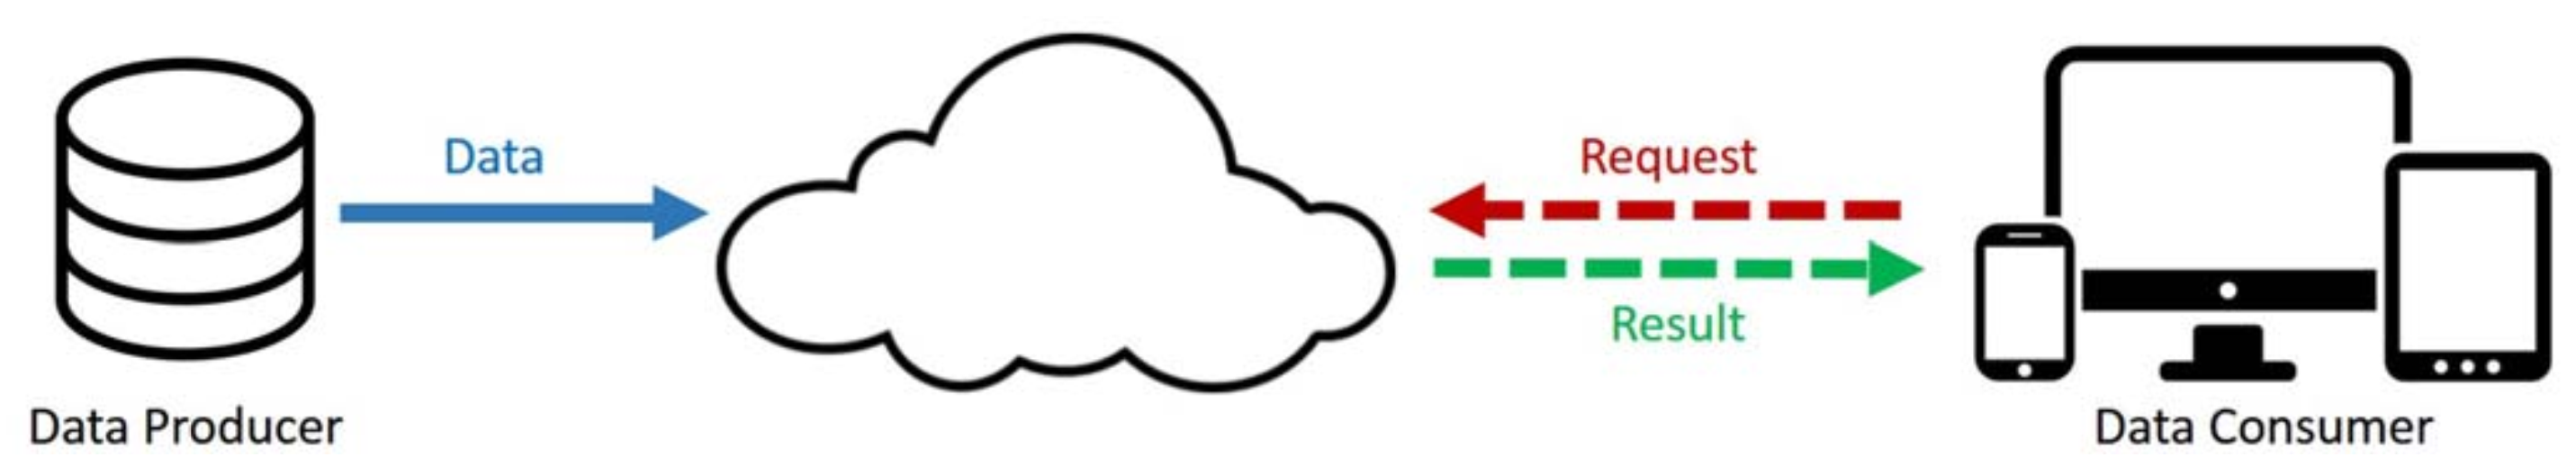
\includegraphics[width=10cm]{graphics/chapter_2/cloud_paradigm}}
            \caption{الگوی پردازش ابری \cite{shi2016edge}}
            \label{fig:chapter_2:cloud_paradigm}
          \end{figure}

        \item [تغییر از مصرف کننده داده به تولید کننده داده:]
          در الگوی پردازش ابری، دستگاه‌های انتهایی در لبه شبکه معمولا نقش مصرف کننده داده را دارند.
          به عنوان نمونه می‌توان تماشای یک ویدیو را مثال زد.
          با این حال امروزه مردم در حال تولید داده توسط دستگاه‌هایشان هستند.
          برای مثال امروزه بسیار عادی است که افراد عکس‌ها و ویدیو‌هایی که توسط خودشان ضبط شده است را در سرویس‌های اینترنتی مختلف به اشتراک بگذارند.
          در \cite{2019domo} اشاره شده است که در هر دقیقه در \lr{twitter} ۵۱۱۲۰۰ توییت جدید ارسال می‌شود و در \lr{instagram} ۵۵۱۴۰ عکس جدید بارگذاری می‌شود.
          باید توجه داشت که این تصاویر و ویدیوها می‌توانند حجم زیادی داشته باشند و پهنای باند زیادی را برای بارگذاری استفاده کنند.
          در این موارد ویدیو‌ها باید ابتدا حجمشان در لبه شبکه کاهش پیدا کند تا به وضوح تصویر\LTRfootnote{Resolution} مناسب برای بارگذاری در شبکه برسند.
          به عنوان نمونه‌ی دیگر می‌توان دستگاه‌های مربوط به سلامت را مثال زد.
          داده‌های جمع‌آوری شده توسط این دستگاه‌ها معمولا خصوصی است و پردازش این داده‌ها در لبه شبکه به جای ارسال داده‌ها برای پردازش به ابر به حفظ حریم خصوصی افراد کمک می‌کند.

      \end{description}
    
    \subsection{پردازش لبه چیست؟}
      پردازش لبه به همه تکنولوژی‌هایی اطلاق می‌شود که امکان انجام پردازش‌ داده‌ها در لبه شبکه را فراهم می‌کنند.
      در اینجا منظور از لبه، همه منابع پردازشی و شبکه ای است که بین منبع داده‌ها (جایی که داده‌ها در آن جا تولید می‌شوند) و مراکز داده‌ی ابری قرار دارند.
      برای مثال یک دروازه‌ی شبکه در یک خانه هوشمند، می‌تواند یک منبع پردازشی لبه بین اشیاء و مرکز داده‌ی ابری باشد یا یک مرکز داده‌ی کوچک، می‌تواند یک منبع پردازشی لبه بین دستگاه‌های سیار و ابر در نظر گرفته شود.
      منطق در پردازش لبه این است که پردازش داده‌ها باید در همسایگی منبع داده‌ها انجام شود.
      با این منطق پردازش لبه و پردازش مه دو مفهوم یکسان را خواهند داشت با این تفاوت که پردازش لبه تمرکزش سمت اشیاء است ولی پردازش مه تمرکزش سمت زیرساخت است.

      \begin{figure}[h]
        \centerline{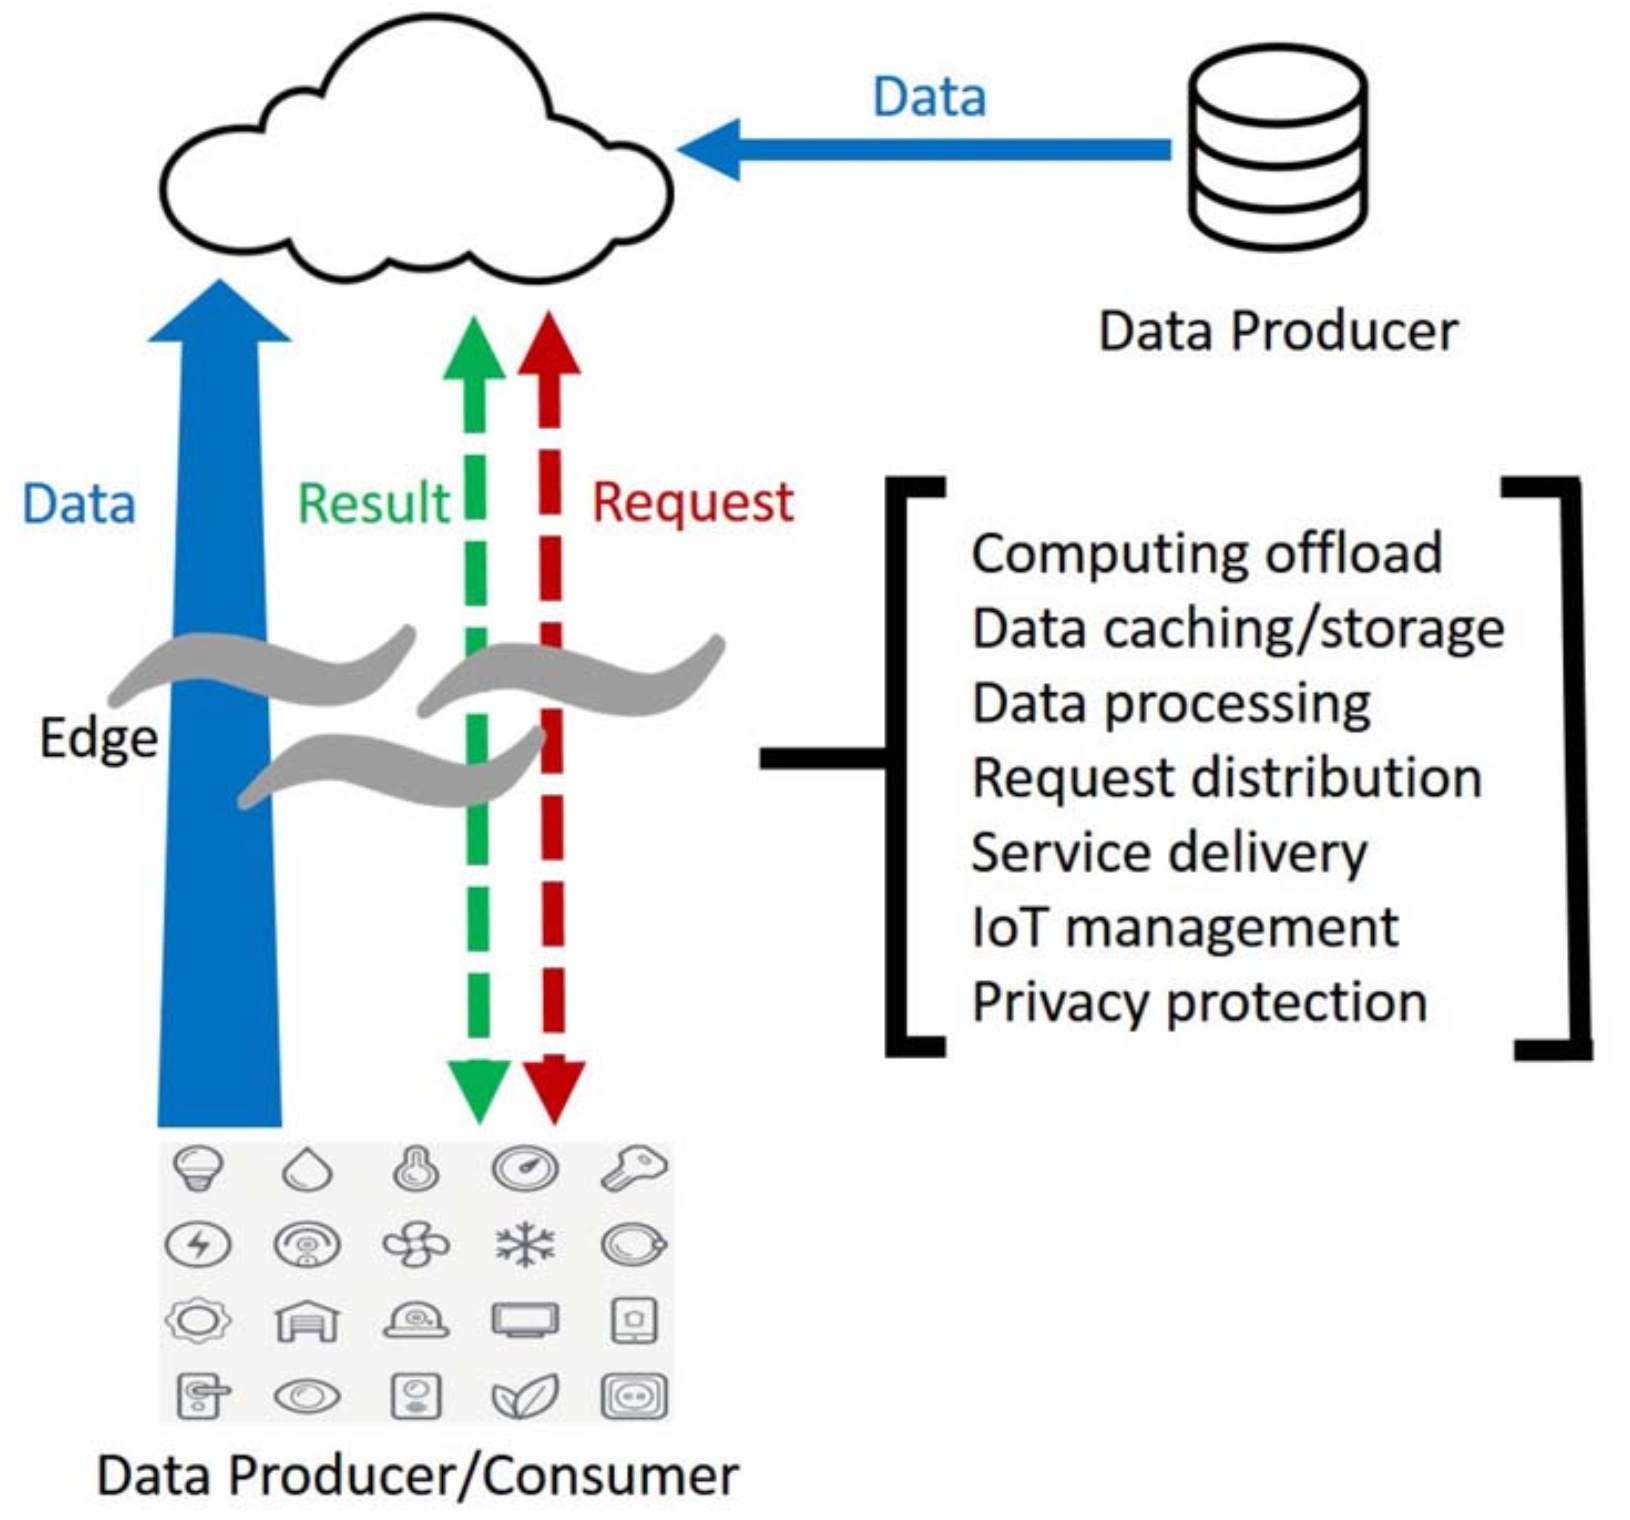
\includegraphics[width=10cm]{graphics/chapter_2/edge_paradigm}}
        \caption{الگوی پردازش لبه \cite{shi2016edge}}
        \label{fig:chapter_2:edge_paradigm}
      \end{figure}
      
      \cref{fig:chapter_2:edge_paradigm} جریان پردازش دو طرفه را در پردازش مه نشان می‌دهد.
      در الگو پردازش لبه، اشیاء نه تنها مصرف کننده داده بلکه تولید کننده‌ داده نیز هستند.
      در واقع در لبه، اشیاء نه تنها می‌توانند سرویس و محتوا از ابر درخواست نمایند بلکه می‌توانند وظایف پردازشی را هم انجام دهند.

    \subsection{مزایای پردازش لبه}
      همان طور که در بخش‌های قبل بیان شد، هدف از پردازش لبه قراردادن پردازش در مجاورت منبع تولید داده‌ها است.
      این کار مزایایی نسبت به روش‌های مبتنی بر پردازش ابری مرسوم دارد.
      در \cite{yi2015fog} برنامه‌ای برای تشخصی چهره ساخته شده است که با انتقال پردازش از ابر به لبه شبکه، زمان پاسخ برنامه از ۹۰۰ به ۱۶۰ میلی ثانیه کاهش پیدا کرده است.
      در \cite{ha2014towards} نویسندگان از واحدهای پردازشی ابری کوچک\LTRfootnote{Cloudlet} برای پردازش وظایف دستیار شناختی پوشیدنی\LTRfootnote{Wearable Cognetive Assitance} استفاده کرده اند و نتایج نشان می‌دهد که زمان پاسخ بین ۸۰ تا ۲۰۰ میلی ثانیه کاهش پیدا کرده است.
      روش ارائه شده در \cite{chun2011clonecloud} برای اجرای برنامه‌های تلفن همراه به کمک استفاده همزمان از پردازش ابری و پردازش لبه توانسته زمان اجرا و انرژی مصرفی را تا ۲۰ برابر کاهش دهد.

    \subsection{کاربرد پردازش لبه در شهر هوشمند}
      ویژگی‌های زیر باعث می‌شوند که پردازش لبه برای استفاده در شهر هوشمند مناسب باشد.
      \begin{enumerate}
        \item \textbf{حجم زیاد داده:}
          تخمین زده می‌شود که در سال ۲۰۱۹ میلادی یک شهر با جمعیت ۱ میلیون نفر، ۱۸۰ پتابایت داده در هر روز تولید می‌کند\cite{index2015forecast}.
          این داده‌ها توسط امنیت عمومی، سلامت، تجهیزات شهری و حمل و نقل تولید می‌شوند.
          ساختن مراکز داده‌ی متمرکز برای رسیدگی به همه‌ی این داده‌ها یک راهکار غیر واقعی است چرا که از این حجم از داده نیاز به قدرت پردازشی بسیار زیادی دارد.
          در این مورد پردازش لبه می‌تواند یک راه حل بهینه برای پردازش این حجم عظیم از داده‌ها باشد.

        \item \textbf{تاخیر کم:}
          برای کاربرد‌هایی که نیاز به تاخیر قابل پیشبینی و کم دارند مانند اورژانس سلامتی و امنیت عمومی، پردازش لبه یک الگوی مناسب است چرا که زمان انتقال داده‌ها را کاهش می‌دهد و ساختار شبکه را ساده‌تر می‌کند
        \item \textbf{آگاهی از مکان:}
          برای کاربرد‌های مبتنی بر موقعیت جغرافیایی مانند حمل و نقل و مدیریت تجهیزات شهری پردازش لبه به دلیل آگاهی از مکان، بهتر از پردازش ابری عمل می‌کند.
      \end{enumerate}

  \section{مجازی سازی}
    در الگوی پردازش ابری برای به اشتراک گذاری منابع از روش‌های مبتنی بر مجازی سازی\LTRfootnote{Virtualization} استفاده می‌شود و فراهم کننده‌های سرویس‌های زیرساخت ابری\LTRfootnote{Cloud Infrastructure as a Service Providers} به کمک این روش‌ها می‌تواند منابع را به صورت سریع به اشتراک بگذارد \cite{pahl2015containers} و \cite{jain2016overview}.
    در پردازش ابری ماشین‌های مجازی \LTRfootnote{Virtual Machine} به عنوان اصلی ترین روش مجازی سازی مورد استفاده قرار می‌گیرند.
    کارآمدی ماشین‌های مجازی در طول زمان با بهبود روش‌های زمان بندی، بسته بندی و ارتقاء امنیت آن‌ها بیشتر شده است.
    هر ماشین مجازی سیستم فایل بندی\LTRfootnote{File System} خود را به عنوان یک فایل مجزا روی حافظه کامپیوتر میزبان ذخیر می‌کند و به عنوان یک پردازه\LTRfootnote{Proccess} بزرگ در کامپیوتر میزبان اجرا می‌شود.
    برای حفظ امنیت هر کدام از این ماشین‌های مجازی، آن‌ها به صورت ایزوله نسبت به هم اجرا می‌شوند.

    در این روش مجازی سازی، هایپروایزر\LTRfootnote{Hypervisor} وظیفه مجازی‌سازی در سطح سخت افزار را دارد.
    به همین دلیل ماشین‌های مجازی از کامپیوتر میزبان مستقل خواهند بود.
    این استقلال از کامپیوتر میزبان باعث می‌شود که ماشین‌های مجازی با سیستم عامل متفاوت از سیستم عامل میزبان قابل اجرا باشند\cite{morabito2015hypervisors}.
    با این حال این روش دارای محدودیت‌هایی هم هست.
    یکی از این محدودیت‌ها این است که تصویر سیستم عامل میزبان به صورت کامل برای تک تک ماشین‌های مجازی نیاز است که باعث مصرف زیاد حافظه ذخیره‌سازی تصادفی و دیسک می‌شود.
    از دیگر محدودیت‌های این روش این است که شبیه سازی دستگاه‌های سخت افزاری توسط هایپروایزر باعث افزایش سربار پردازشی در کامپیوتر میزبان و کاهش بهره‌وری کلی می‌شود.
    علاوه بر این، این روش دارای زمان راه‌اندازی زیادی می‌باشد چراکه سیستم عامل تک تک ماشین‌های مجازی باید راه اندازی شود.
    از هایپروایزرهای مشهور می‌توان \lr{KVM (Kernel Based Virtual Machine)}\cite{2019kvm}, \lr{VMware ESXi}\cite{2019esxi}, \lr{Xen}\cite{2019xen} و \lr{Microsoft Hyper-V}\cite{2019hyper} نام برد.
    \cref{fig:chapter_2:vm} ساختار معماری مبتنی بر هایپروایزر را نشان می‌دهد.

    \begin{figure}[]
      \centerline{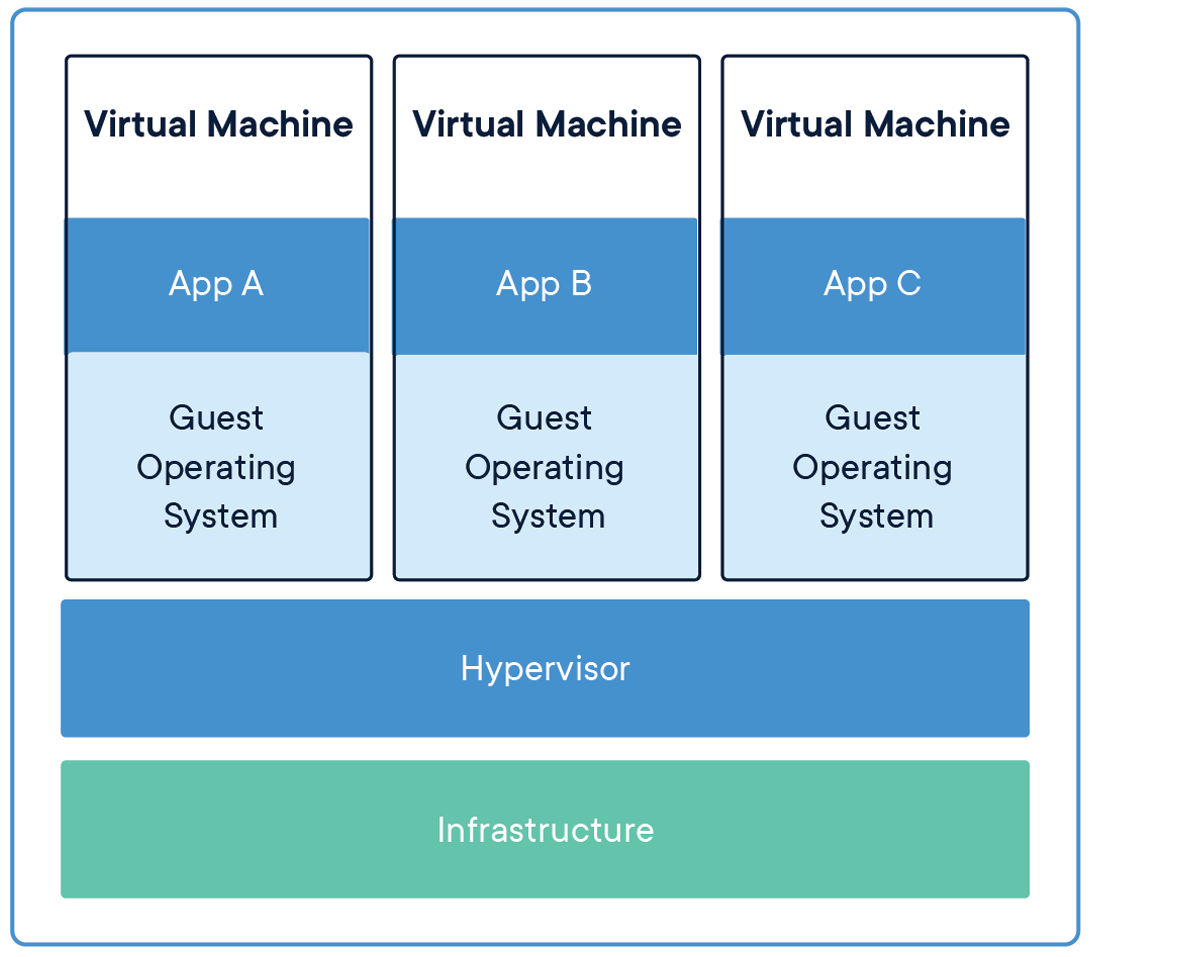
\includegraphics[width=10cm]{graphics/chapter_2/vm}}
      \caption{ساختار معماری مبتنی بر هایپروایزر \cite{2018are}}
      \label{fig:chapter_2:vm}
    \end{figure}

    روش‌های مجازی سازی مبتنی بر کانتینر\LTRfootnote{Container Based 
    Virtualization} مجازی سازی و ایزولاسیون را در سطی متفاوت از سطحی که روش‌های مبتنی بر هایپروایزر انجام می‌دهند، دنبال می‌کنند.
    درواقع می‌توان آن‌ها را جایگزین سبکی برای روش‌های مجازی سازی مبتنی برای هایپروایزر در نظر گرفت.
    در روش‌های مجازی سازی مبتنی بر هایپروایزر یک سیستم عامل مجزا به طور کامل برای هر کدام از ماشین‌های مجازی اجرا می‌شود.
    در مقابل در روش‌های مبتنی بر کانتینر، ایزولایسون پردازه‌ها در سطح سیستم عامل پیاده‌سازی می‌شود.
    برای این کار همه‌ی کانتینر‌ها بر روی یک سیستم عامل مشترک روی کامپیوتر میزبان اجرا می‌شوند و هر کانتینر می‌تواند شامل یک یا چند پردازه باشد.
    بنابراین سربار اجرای چندین سیستم عامل، راه‌انداز‌های سخت افزاری\LTRfootnote{Device Driver} و شبیه‌سازی سخت افزار‌های مختلف را از بین می‌برند.
    ساختار مجازی سازی مبتنی بر کانتیر در \cref{fig:chapter_2:container} نشان داده شده است.

    \begin{figure}[]
      \centerline{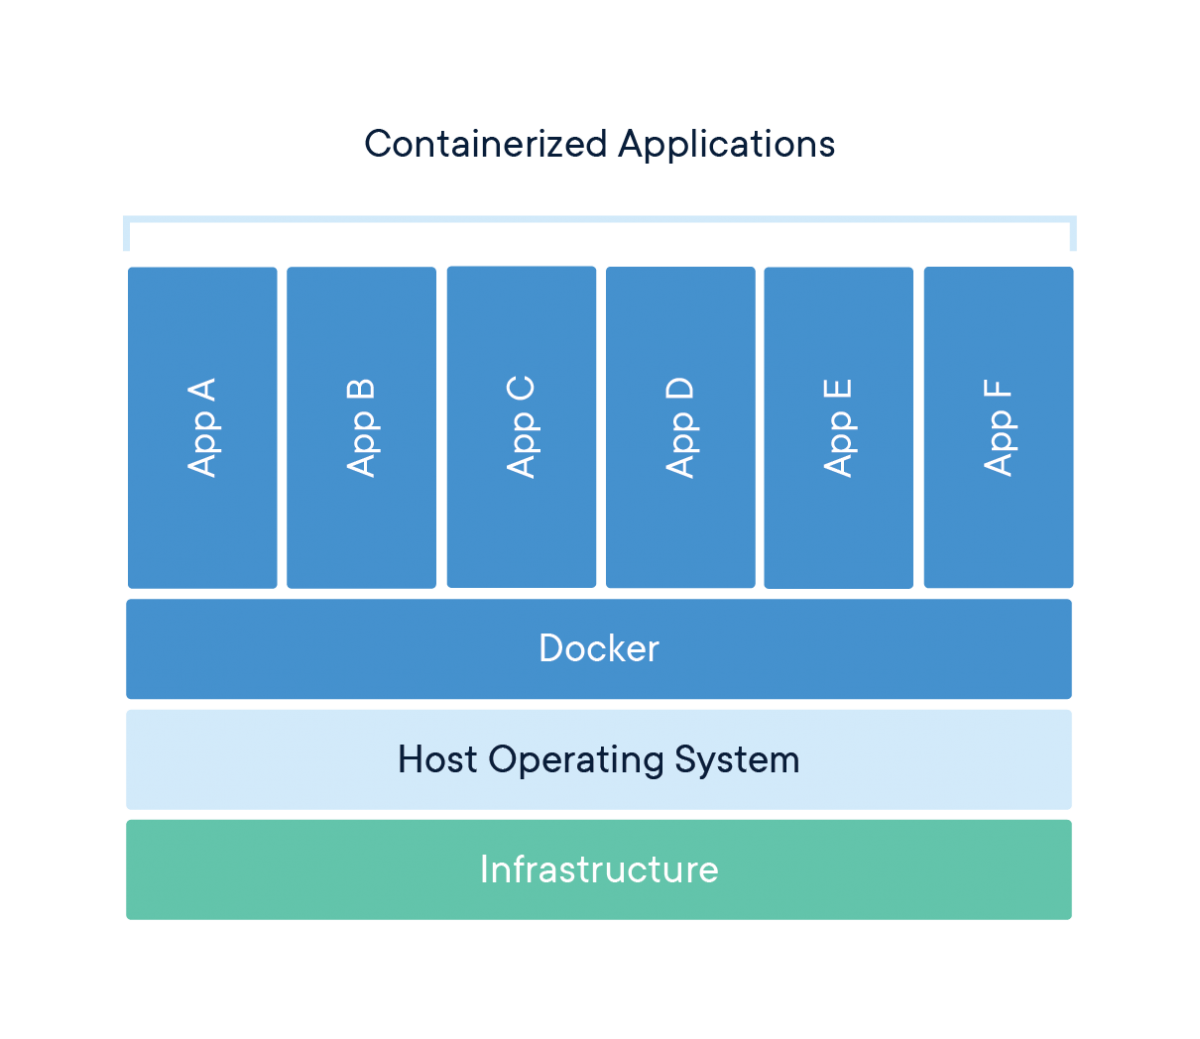
\includegraphics[width=10cm]{graphics/chapter_2/container}}
      \caption{ساختار مجازی سازی مبتنی بر کانتینر \cite{2018are}}
      \label{fig:chapter_2:container}
    \end{figure}
    
    مجازی سازی‌های مبتنی بر کانتینر در مقایسه با روش‌های مجازی سازی سخت افزاری مزایایی مانند سرعت ایجاد سریع‌تر دارند چرا که دیگر نیاز به شروع سیستم‌عامل جداگانه‌ای نیست.
    علاوه بر این سیستم‌های مبتنی بر کانتینر به دیلی حجم کم‌تر  تصویر‌ها\LTRfootnote{Image} و اجرا شدن روی هسته سیستم‌عامل\LTRfootnote{Operating System Kernel} مشترک می‌توانند تخصیص منابع بهتری داشته باشند \cite{morabito2015hypervisors}.

    با این حال استفاده از هسته‌ی سیستم عامل مشترک اشکالاتی در مقایسه با روش‌های مجازی‌سازی مبتنی بر هایپروایزر به همراه دارد.
    یکی از این اشکالات این است که کانتینر‌های سیستم عامل‌های مختلف قابل استفاده در سیستم عامل‌های دیگر نیستند.
    دیگر اشکال مجازی سازی‌های مبتنی بر کانتینر این است که ایزولاسیون در آن‌ها به خوبی روش‌های مجازی سازی مبتنی بر هایپروایزر نیست \cite{bui2015analysis} چرا که هسته سیستم عامل کامپیوتر میزبان در همه کانتینر‌ها مشترک است و این ممکن است برای امنیت در اجاره چندگانه\LTRfootnote{Multi-Tenant} مناسب نباشد.

    در ادامه به بررسی کانتینر‌ها در سیستم عامل لینوکس می‌پردازیم.
    در این سیستم عامل کانتینر‌ها به صورت عمده به وسیله‌ی گروه‌های کنترل\LTRfootnote{Control Groups (cgroups)}\cite{tejun2015Linux} و فضای نام‌ها\LTRfootnote{Name Spaces}\cite{2015Linux} پیاده‌سازی می‌شوند.

    گروه‌های کنترل در سال ۲۰۰۶ توسط مهندسان \lr{Google} توسعه داده‌شد و امکان مدیریت منابع مانند، محدودیت استفاده از منابع یا اولویت پردازه‌ها را برای گروهی از پردازه‌ها مشخص می‌کنند.
    فضای‌نام‌ها هم یک دید محدود و اختصاصی برای منابع سیستم در هر کانتینر ایجاد می‌کند.
    مجموعه‌ای از پردازه‌ها می‌توانند در یک فضای نام قرار بگیرند و محدودیت‌های یکسانی را در استفاده از منابع برای آن‌ها تعریف کرد.
    هر کامپیوتر می‌تواند چندید فضای نام داشته باشد و برای هر کدام ویژگی منابع توسط هسته‌ی سیستم عامل اعمال می‌شود.
    اختصاص منابع به هر فضای نام می‌تواند به گونه‌ای باشد که استفاده از واحد پردازنده مرکزی\LTRfootnote{Central Processing Unit (CPU)}، حافظه‌ی با دسترسی تصادفی\LTRfootnote{Random Access Memory (RAM)} و سایر منابع را برای مجموعه‌ای از پردازه‌ها محدود کند.
    با اضافه شدن ایزولاسیون گروه‌های کنترل در هسته لینوکس امکان ایجاد فضای نام‌هایی که از فضای نام‌های دیگر مستقل باشند ممکن شد.
    چند مورد از مهم‌ترین ویژگی‌های ایزولاسیون در فضای نام‌ها را ادامه بررسی می‌کنیم:
    \begin{enumerate}
      \item \textbf{فضای نام‌های شناسه پردازه‌ها\LTRfootnote{Process Identifier(PID)}:} این ویژگی باعث می‌شود که پردازه‌های یک فضای نام، از پردازه‌های فضای نام‌های دیگر با خبر نباشند.
      \item \textbf{فضای‌نام‌های شبکه:} ایزولاسیون کنترل‌کننده‌های رابط‌های‌ شبکه\LTRfootnote{Network Interface Controller (NIC)}، جدول‌های مسیریابی و ابزار‌های سطح پایین شبکه را ممکن می‌سازد
      \item \textbf{فضای نام‌های دستگاه‌های سوار شده\LTRfootnote{Mount Namespace}:} از این ویژگی برای ایزولاسیون دستگاه‌های سوار شده استفاده می‌شود که باعث می‌شود بتوان روی مصرف فضای نام‌های مختلف از دیسک محدودیت گذاشت.
      \item \textbf{فضای‌نام‌های کاربران:} کاربران یک فضای نام را به همان فضای نام محدود می‌کند و مانع تداخل شناسه‌های کاربری\LTRfootnote{User Identifier (UID)} یکسان در فضای نام‌های مختلف می‌شود.
    \end{enumerate}
    به بیان ساده‌تر این ویژگی‌ها باعث می‌شوند که هر فضای نام به عنوان کامپیوتر میزبان پردازه‌هایی که در آن اجرا می‌شوند ظاهر شود.

    از راه حل‌های مبتنی بر کانتینر می‌توان \lr{Linux-VServer}\cite{2019vserver}، \lr{OpenVZ}\cite{2019openvz}، \lr{LXC}\cite{2019containers}، \lr{Docker}\cite{2019docker} و \lr{rtk}\cite{2019rtk} را نام برد.
    در بین این راه‌حل‌ها \lr{LXC} و \lr{Docker} از بقیه مشهورتر هستند.
    \lr{LXC} یک راه حل سطح پایین‌تر ارائه می‌دهد و زمان زیادی است که موجود است.
    در واقع LXC اولین پیاده‌سازی چیزی که ما امروزه به نام کانتینر می‌شناسیم است.
    \lr{LXC} با استفاده از مزایای گروه‌های کنترل و فضای نام‌ها یک محیط مجازی درست می‌کند که پردازه‌ها به صورت جدا از هم اجرا می‌شوند.
    می‌توان این گونه برداشت کرد که \lr{LXC} امکان وجود فضا‌های کاربری\LTRfootnote{User Space} ایزوله و جدا را روی یک کامپیوتر فراهم می‌کند.
    در مقابل \lr{Docker} در سال ۲۰۰۹ معرفی شد و یک راه حل سطح بالاتر ارائه می‌دهد.
    \lr{Docker} با ترکیب کردن کانتینر‌های لینوکس با یک سیستم فایل‌بندی لایه‌لایه و ارائه ابزار‌هایی برای ساخت و بسته‌بندی برنامه‌های کاربردی به صورت تصویر کانتینر‌ها توانست محبوبیت زیادی کسب کند.
    نخستین نسخه‌های \lr{Docker} به صورت مستقیم از \lr{LXC} استفاده می‌کردند.
    در حال خاضر \lr{Docker} محبوب‌ترین تکنولوژی کانتینر می‌باشد به طوری که بیشتر افراد وقتی از تکنولوژی کانتینر نام برده می‌شود، فقط \lr{Docker} را در نظر می‌گیرند.
    با وجود تکنولوژی‌های مختلف کانتینر که در بالا اشاره شد، \lr{Docker} به عنوان یک استاندارد صنعتی برای کانتینر‌ها پذیرفته شده است.
    با این وجود داکر بر روی گروه‌های کنترل و فضای‌نام‌های هسته لینوکس بنا شده است.

    کانتینر‌های \lr{Docker} از چندین لایه از تصویر‌ها ساخته شده‌اند.
    این تصویر‌ها شامل فایل‌هایی دودویی هستند که باهم در یک بسته‌بندی قرار داده‌ شده‌اند.
    تصویر پایه سیستم عامل کانتینر را نگهداری می‌کند که می‌تواند متفاوت با سیستم عامل کامپیوتر باشد.
    سیستم عامل کانتینر، یک سیستم عامل کامل مانند سیستم عامل کامپیوتر میزبان نیست.
    تفاوت این است که تصویر تنها سیستم فایل بندی و فایل‌های دو دویی سیستم عامل را دارد ولی سیستم عامل کامپیوتر میزبان، سیستم فایل بندی، فایل‌های دو دویی و هسته سیستم عامل را دارا می‌باشد.
    روی تصویر پایه، چندین تصویر قرار می‌گیرد که هر کدام بخشی از کانتینر را می‌سازند.
    در واقع هر تغییری روی فایل‌های تصویر‌های قبلی باعث ایجاد یک لایه جدید می‌شود.
    مزیت این روش این است که باعث کاهش فضای لازم برای نگهداری تصویر کانتینر‌ها می‌شود.
    برای مثال دو کانتینر را با لایه‌های تصویر آ، ب و ث برای کانتینر اول و آ، ب و ت برای کانتینر دوم در نظر بگیرید.
    با این روش نگهداری، لایه‌های تصویر آ و ب تنها یکبار ذخیره می‌گردند ولی اگر تصویر‌ها یکپارچه بودند برای هرکانتینر باید فضا اشغال می‌کردند.

    \begin{figure}[]
      \centerline{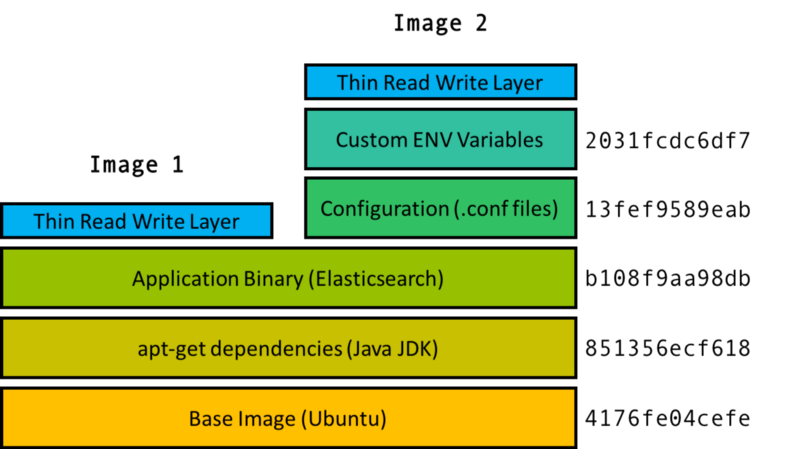
\includegraphics[width=10cm]{graphics/chapter_2/docker_image}}
      \caption{ساختار تصویر کانتینر‌ها در \lr{Docker} \cite{2019demystifying}}
      \label{fig:chapter_2:docker_image}
    \end{figure}

    در \lr{Docker} از نتیجه تابع در هم‌ساز\LTRfootnote{Hash} \lr{SHA-256} روی محتوای هر لایه به عنوان شناسه‌ی آن لایه‌ی تصویر استفاده می‌شود و هر لایه شناسه لایه‌های پایینی خود را نگهداری می‌کند و کانتینر‌ها با شناسه بالاترین تصویرشان متمایز می‌شوند.
    \cref{fig:chapter_2:docker_image}، ساختار تصویر دو کانتینر را نشان می‌دهد.
    همان طور که مشخص است این دو تصویر دارای سه لایه مشترک هستند و تصویر ۲ دارای دو لایه اضافی نیز هست.
    هنگامی که کانتینر اجرا می‌شود، \lr{Docker} ابتدا همه‌ی لایه‌های تصویر‌ها را بارگیری می‌کند.
    سپس گروه کنترل و نام‌دامنه‌های مربوط به کانتینر جدید را ایجاد می‌کند و از تصویر برای ایجاد محیط مجازی استفاده می‌کند به طوری که برای پردازه‌هایی که در آن کانتینر اجرا می‌شوند، انگار که فقط فایل‌های تصویر روی کامپیوتر قرار دارند.
    در انتها پردازه اصلی کانتینر را اجرا می‌کند.

    در \cite{ismail2015evaluation} نویسندگان، \lr{Docker} را به عنوان تکنولوژی که امکان استفاده از پردازش لبه را فراهم می‌کند بررسی کرده‌اند.
    نویسندگان، \lr{Docker} را در زمینه‌ی استقرار و پایان دادن سرویس‌ها، مدیریت منابع و سرویس‌ها، تحمل خطا و ذخیره‌سازی مورد بررسی قرار دادند و نتیجه گرفتند که \lr{Docker} به عنوان یک راه حل مناسب برای استفاده در پردازش لبه قابل استفاده است.
    در \cite{viswanath2016system} و \cite{morabito2016enabling} از تکنولوژی‌های مجازی‌سازی سبک برای طراحی دروازه‌های\LTRfootnote{Gateway} اینترنت اشیاء استفاده شده است.
    در \cite{viswanath2016system} از یک نرم‌افزار مجازی سازی برای استقرار انبوه سرویس‌ها در لبه شبکه استفاده کرده‌اند.
    نکته قابل توجه در تحلیل آن‌ها، امکان اثر متقابل بین حسگر‌های اینترنت اشیاء و دروازه‌‌ها می‌باشد.
    تحلیل آن‌ها نشان می‌دهد که تخصیص پویای سرویس‌ها با استفاده از کانتینر‌ها مزایایی از بعد کارایی در دروازه‌ها دارد.
    در \cite{morabito2016enabling} یک طراحی برای دروازه‌های اینترنت اشیاء ارائه شده است که می‌تواند به صورت بهینه در لبه شبکه استفاده شود.
    بررسی‌های انجام‌شده در این مقاله کارآمدی و انعطاف پذیری استفاده از \lr{Docker} را برای استفاده در یک سکوی‌ اینترنت اشیاء که سرویس‌های مجازی مختلفی مانند مدیریت دستگاه‌ها، پشتیبانی از شبکه‌های مبتنی بر نرم‌افزار\LTRfootnote{Software Defined Network (SDN)} و امکان مدیریت و ساماندهی داده‌ها را ارائه دهد، نشان می‌دهد.

    در \cite{novo2015capillary} از \lr{Docker} برای بسته‌بندی، استقرار و اجرای نرم‌افزار‌ها در ابر و دستگاه‌های با منابع محدود مانند دروازه‌های خاصی استفاده شده است.
    هدف این دروازه‌ها فراهم کردن اتصال شبکه‌های با برد کوتاه با شبکه‌های سلولی و فراهم کردن اجزاء نرم‌افزار‌های مختلف برای مدیریت دستگاه‌ها و پردازش‌های ابری توزیع‌شده می‌باشد.
    در \cite{celesti2016exploring} مجازی سازی مبتنی بر کانتینر و کامپیوتر‌های تک بردی\LTRfootnote{Single Board Computer (SBC)} به عنوان تکنولوژی‌هایی که امکان فراهم سازی سرویس‌های اینترنت اشیاء ابری را مهیّا می‌کنند، شناخته شده‌اند.
    مقاله \cite{krylovskiy2015internet} به شناسایی و بررسی نیازمندی‌های طراحی دروازه اینترنت اشیاء پرداخته است.
    نویسندگان کانتینر‌های \lr{Docker} را به عنوان تکنولوژی مناسب که این نیازمندی‌ها را برطرف می‌کند در نظر گرفتند.
    در این مطالعه، برای برآورد سربار لایه مجازی سازی از چند معیار ترکیبی و کاربردی استفاده شده است.
    با این حال، در این مطالعه، کارایی فقط برای برد \lr{Raspberry Pi} انجام شده و بررسی جامع مصرف توان و بهره‌وری انرژی در آن وجود ندارد.

    معماری ابر کوچک که در \cite{satyanarayanan2009case} معرفی شده است، یک روش کارآمد برای پردازش ابری سیار\LTRfootnote{Mobile Cloud Computing} ارائه می‌دهد که برخلاف مقالات قبلی از ماشین مجازی برای مجازی سازی استفاده کرده است.
    در \cite{pahl2016container} نویسندگان یک سکوی به عنوان سرویس\LTRfootnote{Platform as a Service (PaaS)} مبتنی بر کانتینر با استفاده از \lr{Raspberry Pi} معرفی کرده‌اند که در آن از تکنولوژی‌های کانتینری برای استفاده در معماری ابری لبه استفاده شده است.
    به طور مشابه در \cite{bellavista2017feasibility} از \lr{Docker} و \lr{Raspberry Pi} برای ایجاد یک شبکه پردازش لبه استفاده کرده‌اند.
    نویسندگان سربار استفاده از \lr{Docker} برای کامپیوتر‌های تک بردی را بررسی کرده و آن را ناچیز ارزیابی کرده‌اند.
    \cite{hajji2016understanding} به بررسی جزئی کارایی یک معماری ابری مبتنی بر \lr{Raspberry Pi} و \lr{Docker} برای استفاده در کاربرد‌های کلان داده\LTRfootnote{Big Data} می‌پردازد.
    در انتها، \cite{morabito2017virtualization} به بررسی کارآیی تکنولوژی‌های کانتینری روی کامپیوتر‌های تک بردی مختلف می‌پردازد.
    در همه این مقالات نتیجه گیری بر این است که با استفاده از کانتینر‌ها در دستگاه‌های مورد نظر، سربار پردازشی قابل چشم پوشی می‌باشد.

  \section{نو‌آوری‌های پایان نامه}
    دستاورد‌های این پایان‌نامه را می‌توان به صورت زیر خلاصه کرد:

    در بخش اول، برای صورت مسئله تخصیص منابع به صورت یک سرویس به یک منبع پردازشی، مدل ریاضی ارائه شده‌است و مسئله به صورت یک بهینه سازی نوشته شده‌است که هدف آن کمینه کردن مجموع هزینه سرویس‌ها است. برای حل این مسئله یک روش تخصیص منابع مبتنی بر مزایده استفاده است که امکان حل این مسئله به صورت موازی را دارد که برای شبکه‌های بزرگ مناسب است.

    در بخش دوم، برای صورت مسئله تخصیص منابع به صورت چند سرویس به چند منبع پردازشی، مدل ریاضی ارائه شده و به صورت یک مسئله بهینه سازی فرمول بندی شده که نرخ ارسال داده‌ی حسگر‌ها و بیشترین تاخیر سرویس را در تابع هزینه سرویس‌ها دخیل می‌کند و مجموع هزینه سرویس‌ها را کمینه می‌کند.
    ارائه الگوریتم برای حل این مسئله و بررسی تاثیر نرخ انتخابی در تاخیر سرویس‌ها از دیگر نو‌آوری‌های این پایان نامه است.

  \section{ساختار پایان‌نامه}
    ساختار پایان‌نامه به شرح زیر است.

    \cref{chap:literature_review} به مروری بر مطالعات انجام شده در زمینه تخصیص منابع اینترنت اشیاء می‌پردازد.

    \cref{chap:one_to_one_allocation} به بررسی مسئله اختصاص منابع پردازشی به صورت یک به یک در شبکه اینترنت اشیاء اختصاص دارد.
    در این فصل فرض بر این است که سرویس‌ها، می‌توانند از یک منبع پردازشی استفاده کنند و منابع پردازشی هم می‌توانند به یک سرویس اختصاص پیدا کنند.
    تخصیص منابع به صورت یک مسئله بهینه سازی فرمول بندی می‌شود که حل بهینه‌ی آن پیچیده است.
    برای حل مسئله از یک روش مبتنی بر مزایده استفاده شده که جواب قابل قبولی برای مسئله ارائه می‌دهد.

    در \cref{chap:many_to_many_allocation} مسئله تخصیص منابع پردازشی به صورت چند به چند در شبکه اینترنت اشیاء مورد بررسی قرار گرفته است.
    در این فصل بر خلاف فصل قبل منابع پردازشی می‌توانند به چند سرویس اختصاص پیدا کنند و سرویس‌ها هم می‌توانند از چند منبع پردازشی استفاده کنند.
    مانند فصل قبل مسئله تخصیص منابع به صورت یک مسئله بهینه سازی فرمول‌بندی شده است که حل بهینه پیچیده‌ای دارد و برای حل آن الگوریتمی پیشنهاد شده که در زمان کوتاه‌تری مسئله را حل می‌کند.

    در انتها در \cref{chap:conclusion} به بیان نتیجه‌گیری و کار‌های آینده می‌پردازیم.
